% ------------------------------------------------------------------------------
% The implemtations shows specifically how your research was conducted.
% All the impementation details and practical tests can be listed.
% ------------------------------------------------------------------------------

\opt{never}{\addbibresource{03-tail/bibliography.bib}} % to make citation found in most IDE

\chapter{Implementation}
\label{chap:implementation}

% -- Your text goes here --
The implementation sets out the concrete realisation of the reference architecture, detailing the tools used to automate the deployment of the \gls{cloud_infrastructure} and the integration of the embedded systems. Particular attention is paid to the in-depth description of the automated pipeline. The various applications that accompany this architecture are also highlighted.

\minitoc
\newpage

% ------------------------------------------------------------------------------
\section{Reference architecture}

% -- Your text goes here --
\subsection{\Gls{cloud_infrastructure}}
An \acrfull{iac} tool was selected to orchestrate the efficient deployment of the \gls{cloud_infrastructure} on \gls{aws}, and Pulumi was chosen because of its choice of programming language, in this case Python. The use of the same programming language for the implementation of applications and the description of \gls{aws} resources provides consistency within the project.

Integrating Pulumi is simple. The resources required are described in Python files. The deployment is managed by the Pulumi \acrshort{cli}, which records the state of the infrastructure in an Amazon S3 compartment. This compartment is located in the same \gls{aws} account as the infrastructure, using Amazon S3 to store the state rather than the default Pulumi \Gls{cloud} platform, thus eliminating external dependencies. Figure \ref{fig:pulumi_overview} shows an overview of this part of the implementation.
\begin{center}
    \begingroup
    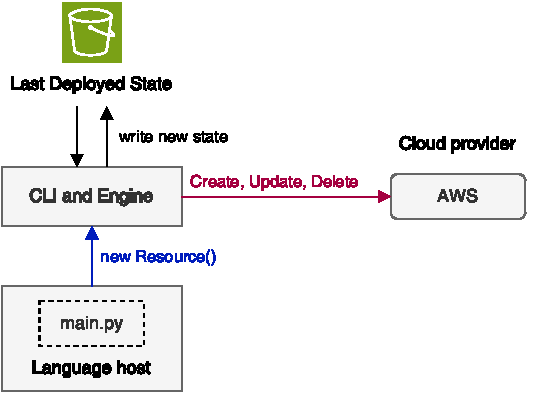
\includegraphics[width=.7\columnwidth]{implementation/pulumi_overview.pdf}
    \captionof{figure}{Overview of Pulumi's integration into the reference architecture}
    \label{fig:pulumi_overview}
    \endgroup
\end{center}
This \gls{cloud_infrastructure} part is implemented in a specific folder as follows :
\begin{center}
    \usemintedstyle{pastie}
    \begin{minted}
    [
    fontsize=\scriptsize
    ]{text}
    cloud-infrastructure
        ├── Pulumi.yaml
        ├── Pulumi.dev.yaml
        ├── Pulumi.prod.yaml
        ├── main.py
        ├── iam.py
        └── requirements.txt
    \end{minted}
\end{center}
The main configuration file for the Pulumi tool, \textit{Pulumi.yaml}, includes crucial information such as the name of the stack and the programming language used, in this case Python.

This implementation aims to facilitate the deployment of two distinct infrastructures, namely the development environment and the production environment. Therefore, two additional configuration files, \textit{Pulumi.dev.yaml} and \textit{Pulumi.prod.yaml}, are present to differentiate these two environments. \textit{Pulumi.dev.yaml} contains parameters such as the \gls{aws} development account ID and the deployment region, while \textit{Pulumi.prod.yaml} includes the same parameters with production-specific values. The identifiers of the \gls{aws} accounts must be different.

The Python files \textit{main.py} and \textit{iam.py} detail the description of the resources to be deployed. \textit{iam.py} focuses on IAM roles and policies, while \textit{main.py} mainly covers resources related to \acrshort{iot} and other resources.

Finally, the \textit{requirements.txt} file lists the Pulumi libraries to be installed, including the main Pulumi library, which is essential for all \acrshort{iac} projects.

In terms of the Pulumi libraries used, \gls{aws} Native, a new preview, uses the \gls{aws} \Gls{cloud} Control API to manage and provision \gls{aws} resources, generally aligning with the latest \gls{aws} features as they are released. The resources available in this library are based on those defined in the \gls{aws} CloudFormation registry. In addition, \gls{aws} Classic is another library that is used to fill in resources that are not yet available in \gls{aws} Native. This library uses the \gls{aws} SDK to manage and provision these resources.


\subsection{Embedded systems integration}
\subsubsection{\gls{aws} \acrshort{iot} Greengrass}
Integrating embedded systems with the \gls{aws} ecosystem is crucial to reaping the full benefits of \hyperref[subsec:cloudcomputing]{cloud computing}. To this end, \gls{aws} \acrshort{iot} Greengrass was chosen, a powerful solution that facilitates the execution of local processing on \acrshort{iot} devices, while enabling seamless interaction with \gls{aws} \gls{cloud} services. \gls{aws} defined this solution as follows :
\begin{quote}
    \textit{\gls{aws} \acrshort{iot} Greengrass is an open source \acrfull{iot} edge runtime and \gls{cloud} service that helps you build, deploy and manage \acrshort{iot} applications on your devices. You can use \gls{aws} \acrshort{iot} Greengrass to build software that enables your devices to act locally on the data that they generate, run predictions based on machine learning models, and filter and aggregate device data. \gls{aws} \acrshort{iot} Greengrass enables your devices to collect and analyze data closer to where that data is generated, react autonomously to local events, and communicate securely with other devices on the local network. Greengrass devices can also communicate securely with \gls{aws} \acrshort{iot} Core and export \acrshort{iot} data to the \gls{aws} Cloud. You can use \gls{aws} \acrshort{iot} Greengrass to build edge applications using pre-built software modules, called components, that can connect your edge devices to \gls{aws} services or third-party services. You can also use \gls{aws} \acrshort{iot} Greengrass to package and run your software using Lambda functions, Docker containers, native operating system processes, or custom runtimes of your choice. \cite{aws_iot_greengrass}}\\
\end{quote}
In this implementation, \gls{aws} \acrshort{iot} Greengrass Core software is deployed on embedded systems, acting as an intelligent hub that manages interactions with the \gls{aws} \gls{cloud}. It adapts perfectly to Linux \acrshort{os}. Greengrass components, encapsulating the necessary code, dependencies and resources, are then deployed automatically using mechanisms such as \gls{aws} \acrshort{iot} Greengrass Deployment.

A component must be installed. \textit{Greengrass nucleus} (aws.greengrass.Nucleus) is a mandatory component and the minimum requirement for running \gls{aws} \acrshort{iot} Greengrass Core software on a device. It is configurable to customize and update the \gls{aws} \acrshort{iot} Greengrass Core software \acrlong{ota}.

\subsubsection{Communication}
In this project, components running on an embedded system use the \gls{aws} \acrshort{iot} Greengrass Core \acrfull{ipc} library, available in the \gls{aws} \acrshort{iot} Device SDK, to exchange data with the \gls{aws} \acrshort{iot} Greengrass nucleus and other Greengrass components. The \acrshort{ipc} interface supports the \acrlong{mqtt} communication protocol. \acrshort{mqtt} offers lightweight, asynchronous communication.

Publish/subscribe messaging allows messages to be sent and received in topics. Components can publish messages in topics to communicate with other components, and those who have subscribed to the topic can act on messages received. In this case, the communication is local to the \acrshort{iot} device.

The \acrshort{ipc} interface also facilitates the sending and receiving of \acrshort{mqtt} messages between \gls{aws} \acrshort{iot} Greengrass and \gls{aws} \acrshort{iot} Core. Components can publish messages to \gls{aws} \acrshort{iot} Core and subscribe to topics to react to \acrshort{mqtt} messages from other sources.

\subsubsection{\acrshort{ota} update}
All devices with \gls{aws} \acrshort{iot} Greengrass Core software can obtain \acrshort{ota} updates via \acrshort{mqtt}.

\textbf{\gls{aws} \acrshort{iot} Greengrass Core software update}\\
This functionality is built into the \gls{aws} \acrshort{iot}Greengrass Core software. It is made possible by the \textit{Greengrass nucleus} component and other optional components. The following information is taken from the \gls{aws} documentation \cite{ota_aws_iot}.

A few prerequisites must be met before an update can be carried out. Firstly, the Greengrass device must be connected to the \gls{cloud} \gls{aws} in order to receive the deployment. It must be properly configured with certificates and authentication keys to interact with both the \gls{aws} \acrshort{iot} Core and \gls{aws} \acrshort{iot} Greengrass. Finally, the \gls{aws} \acrshort{iot} Greengrass Core software must be configured and run as a system service.

There are a few things to bear in mind when upgrading. The Greengrass nucleus stops. This stops all the other components present. When the nucleus component is shut down, the device's connection to \gls{aws} is lost.

The following table summarises the behaviour of Greengrass updates :

\begin{tabularx}{1\textwidth} { 
    | >{\raggedright\arraybackslash}X 
    | >{\raggedright\arraybackslash}X 
    | >{\raggedright\arraybackslash}X | }
    \hline
    \rowcolor{lightgray}
    Action              & Deployment configuration  & Nucleus update behavior \\ \hline
    \multirow{2}{\linewidth}{Add new devices to a thing group targeted by an existing deployment without revising the deployment.}
    & The deployment does not directly include Greengrass nucleus.
    
    The deployment directly includes at least one AWS-provided component, or includes a custom component that depends on an AWS-provided component or on the Greengrass nucleus.
    & On new devices, installs the latest patch version of nucleus that meets all component dependency requirements.

    On existing devices, does not update the installed version of the nucleus. \\ \cline{2-3}
    & The deployment directly includes a specific version of the Greengrass nucleus.
    & On new devices, installs the specified nucleus version.

    On existing devices, does not update the installed version of the nucleus. \\ \hline
    \multirow{2}{\linewidth}{Create a new deployment or revise an existing deployment.}
    & The deployment does not directly include Greengrass nucleus.

    The deployment directly includes at least one AWS-provided component, or includes a custom component that depends on an AWS-provided component or on the Greengrass nucleus.
    & On all targeted devices, installs the latest patch version of the nucleus that meets all component dependency requirements, including on any new devices that you add to the targeted thing group. \\ \cline{2-3} 
    & The deployment directly includes a specific version of the Greengrass nucleus.
    & On all targeted devices, installs the specified nucleus version, including any new devices that you add to the targeted thing group. \\ \hline
\end{tabularx}

In this reference architecture, the version of \textit{Greengrass nucleus} is not specified. However, there is one component provided by \gls{aws} (\textit{aws.greengrass.Cli}) and custom components which depend on several components provided by \gls{aws}.

\textbf{Greengrass components update}\\
For custom or public \gls{aws} components, the \gls{aws} \acrshort{iot} Greengrass Deployment service enables OTA updates.

The prerequisites for an update are the same as for the software update. When an update is deployed, only components with a new version are updated. These components will then be stopped and restarted automatically after being updated. If a deployment error occurs, a rollback is performed and the components resume their course with the old version.

The following table explains two main actions:

\begin{tabularx}{1\textwidth} { 
    | >{\raggedright\arraybackslash}X
    | >{\raggedright\arraybackslash}X | }
    \hline
    \rowcolor{lightgray}
    Action              & Components behaviour \\ \hline
    Add new devices to a group of devices targeted by an existing deployment without modifying the deployment.
    & All the components and dependencies present in the deployment are automatically deployed with their latest version on the new devices.
    
    On existing devices, nothing happens.\\
    \hline
    Create a new version of one or more Greengrass components.
    & Only components with a new version will be deployed on all devices in the group of devices targeted for deployment. \\
    \hline
\end{tabularx}

\subsubsection{Fleet \gls{provisioning}}
With \gls{aws} \acrshort{iot} fleet \gls{provisioning}, it is possible to securely set up \gls{aws} \acrshort{iot} to generate and distribute X.509 device certificates and private keys to each device when they first connect to \gls{aws} \acrshort{iot} \cite{aws_iot_greengrass_fleet}. These client certificates, signed by the Amazon Root Certificate Authority, are provided by \gls{aws} \acrshort{iot}. It is very flexible to define specific device groups, device types and permissions for Greengrass Core devices to be provisioned using fleet \gls{provisioning}. A \gls{provisioning} template is used to describe the \gls{provisioning} process for each device, detailing the device, policy and certificate resources to be created during \gls{provisioning}. This template is created from Pulumi.

\gls{aws} \acrshort{iot} Greengrass offers a dedicated \gls{aws} \acrshort{iot} fleet \gls{provisioning} plugin (\textit{aws.greengrass .FleetProvisioningByClaim}), which facilitates the installation of \gls{aws} \acrshort{iot} Greengrass Core software using the resources created by \gls{aws} \acrshort{iot} fleet \gls{provisioning}. This plugin uses claim-based \gls{provisioning}, where devices use a \gls{provisioning} claim certificate and private key to obtain a unique X.509 device certificate, along with a private key, enabling regular operations. The claim certificate and private key are integrated as soon as the Linux \acrshort{os} image is created, enabling devices to be activated later when they are connected. The same claim certificate and private key can be used for multiple devices.

To deploy \gls{aws} \acrshort{iot} Greengrass Core software with \gls{aws} \acrshort{iot} fleet provisioning, configuration of resources in the \gls{aws} account is required. These resources include a provisioning template, a claim certificate and a token exchange IAM role. Once these elements have been created from Pulumi, apart from the certificate from the \gls{aws} \acrshort{cli}, they can be reused to provision several embedded systems within the same fleet. The token exchange IAM role authorises calls to \gls{aws} services from the \acrshort{iot} device.

In this architecture, devices are registered by their serial number to ensure that each one has a unique name.

\subsubsection{\acrshort{os} image}
To enable the devices to be provisioned to integrate automatically on their first boot, a Linux \acrshort{os} image is created specifically for this purpose. The base image used for this architecture is \textit{Raspberry Pi \acrshort{os} Lite} based on the Debian distribution. A directory dedicated to the creation of the image is present as follows:
\begin{center}
    \usemintedstyle{pastie}
    \begin{minted}
    [
    fontsize=\scriptsize
    ]{text}
    os-image
        ├── raspios-lite.json
        ├── set_os.sh
        ├── provision.sh
        └── config.yaml
    \end{minted}
\end{center}
Image creation is managed by Packer \cite{packer}, an open source tool for automating image creation. Packer follows a process defined in a configuration file \acrshort{json} (\textit{raspios-lite.json}).

It works as follows :
\begin{enumerate}
    \item \textbf{Packer configuration} (raspios-lite.json) : The Packer configuration file describes all the steps required to create the image. It specifies the constructors (in this case, the Arm constructor), the actions to be performed, the base image sources and other parameters.
    \item \textbf{Running Packer} : In this project, Packer runs in a Docker environment. When the container is launched, the tool starts the build process following the specified configuration.
    \item \textbf{Packer builder ARM plugin} : A plugin \cite{packer_plugin} to the Packer tool is used to build images specific to the Arm architecture. It uses the Arm build model to create a custom image based on the specification.
    \item \textbf{Actions} : The actions in the configuration file are carried out to configure the image. This may involve installing software, configuring system parameters, etc. In this case, some system parameters are configured using the \textit{set\_os.sh} script. The \gls{provisioning} script \textit{provision.sh} used to install the necessary software is saved in the image and configured to run the first time the operating system is booted. Finally, the claim certificate and its private key are saved in the image.
    \item \textbf{Build complete} : Once all the build and configuration steps have been successfully completed, Packer creates a custom image in the specified format (.img in this case).
\end{enumerate}

The \gls{provisioning} file \textit{provision.sh} is a bash script. When it first runs on a device, it first retrieves the device's serial number, so that the device is registered in \gls{aws} \acrshort{iot} under that name. The script then installs the Docker Engine software, paving the way for future deployment of Greengrass components in containers. After this step, \gls{aws} \acrshort{iot} Greengrass Core is installed with the plugin specially dedicated to fleet \gls{provisioning}. Finally, the \gls{provisioning} command is executed using the \textit{config.yaml} configuration file, which contains various parameters such as the device serial number, as well as the paths to locate the claim certificate and private key.

\subsection{Security}
At \gls{aws}, security is a top priority \cite{aws_iot_greengrass_security}. Security is a shared responsibility between \gls{aws} and the developer :
\begin{itemize}
    \item \textbf{Security of the \gls{cloud}} : \gls{aws} is responsible for protecting the infrastructure that runs \gls{aws} services in the \gls{aws} \gls{cloud}.
    \item \textbf{Security in the \gls{cloud}} : The developer's responsibility is determined by the \gls{aws} service that he uses.
\end{itemize}
When using \gls{aws} \acrshort{iot} Greengrass, the developer is also responsible for securing these devices, the connection to the local network and the private keys.

\subsubsection{Authentication}
Greengrass devices use X.509 certificates for authentication. X.509 certificates are digital certificates that adopt the X.509 public key infrastructure standard to bind a public key to the identity specified in the certificate. These X.509 certificates are issued by a trusted entity known as a \acrfull{ca}. The \acrshort{ca} holds one or more specific certificates, called \acrshort{ca} certificates, which it uses to issue X.509 certificates. Only this \acrshort{ca} has the privilege of accessing the certificates. In this process, the authority is Amazon Root \acrlong{ca}. When \gls{provisioning} a device, the fleet \gls{provisioning} plugin requests a unique client certificate from this authority. \cite{aws_iot_greengrass_security}

Only devices authorised to be provisioned will receive a certificate. In this implementation, a list allowing the serial numbers of authorised devices to be inserted has been created in a dedicated file (\textit{allowlist.txt}). When the \gls{provisioning} plugin attempts to provision a device, it will first trigger a Lambda function which will check the list to see if the device is authorised. If so, it will receive its unique certificate. If not, it will not receive it and will not be provisioned.

Greengrass devices store certificates in the default Greengrass root folder (\textit{/v2/greengrass/}).

\subsubsection{Authorization}
Greengrass devices rely on \gls{aws} \acrshort{iot} policies for authorization. These \gls{aws} \acrshort{iot} policies determine the scope of operations permitted for \gls{aws} \acrshort{iot} devices. They specify, in detail, permissions or denials of access to \gls{aws} \acrshort{iot} Core and \gls{aws} \acrshort{iot} Greengrass data plane operations, including actions such as publishing \acrshort{mqtt} messages. In this architecture, an \gls{aws} \acrshort{iot} policy is created directly from Pulumi. \cite{aws_iot_greengrass_security}

\subsubsection{Data protection}
Greengrass devices frequently collect data for transmission to \gls{aws} services for further processing. \gls{aws} \acrshort{iot} Greengrass uses encryption to protect data in transit (via the internet or local network) and at rest (stored in the \gls{aws} \gls{cloud}). \cite{aws_iot_greengrass_security}

\gls{aws} \acrshort{iot} Greengrass offers two distinct modes of communication for data in transit :
\begin{itemize}
    \item \textbf{Data in transit over the internet} : Communication over the internet between a device and \gls{aws} \acrshort{iot} is encrypted using the \acrfull{tls} protocol. \acrshort{tls} is a security protocol that guarantees the confidentiality and integrity of data when it is exchanged over a network. All data sent to the \gls{aws} \gls{cloud} therefore uses the \acrshort{mqtt} protocol based on \acrshort{tls}.
    \item \textbf{Data on the device} : Communication between components on the Greengrass device is not encrypted, as the data does not leave the device.
\end{itemize}

When it comes to data at rest, \gls{aws} \acrshort{iot} Greengrass adopts different approaches :
\begin{itemize}
    \item \textbf{Data at rest in the \gls{aws} \gls{cloud}} : Customer data stored in the \gls{aws} \gls{cloud} is encrypted by the \gls{aws} \acrshort{iot} Greengrass service using \gls{aws} KMS keys under its management.
    \item \textbf{Data at rest on the Greengrass device} : Data at rest on the device is protected by Unix file permissions and full disk encryption (if enabled, not enabled in this implementation). The user is responsible for securing the file system and the device.
\end{itemize}